\chapter{Задание 1. Спектральное дифференцирование}
\label{ch:chap1}

\definecolor{codegreen}{rgb}{0,0.6,0}
\definecolor{codegray}{rgb}{0.5,0.5,0.5}
\definecolor{codepurple}{rgb}{0.58,0,0.82}
\definecolor{backcolour}{rgb}{0.95,0.95,0.92}

\lstdefinestyle{mystyle}{
    backgroundcolor=\color{backcolour},   
    commentstyle=\color{codegreen},
    keywordstyle=\color{magenta},
    numberstyle=\tiny\color{codegray},
    stringstyle=\color{codepurple},
    basicstyle=\ttfamily\footnotesize,
    breakatwhitespace=false,         
    breaklines=true,                 
    captionpos=b,                    
    keepspaces=true,                 
    numbers=left,                    
    numbersep=5pt,                  
    showspaces=false,                
    showstringspaces=false,
    showtabs=false,                  
    tabsize=2
}

\lstset{style=mystyle}

\section{Лирическое вступление}

В данном задании мы рассматриваем сигнал \texttt{y=sin(t)} с небольшим шумом уже знакомого вида - \texttt{a*(rand(size(t))-0.5)}

Для начала найдём численную производную от зашумлённого сигнала через поэлементную формулу: $$\frac{y(k+1) - y(k)}{dt}$$

Найдём численную спектральную производную от зашумлённого сигнала, использую свойство Фурье-оператора: $$\mathbb{F}(\frac{df}{dt}) = 2\pi i \nu\mathbb{F}(f)$$

То есть, сначала мы получаем Фурье-образ от обычного сигнала, потом домнажаем поэлементно на константы, это нас сразу сводит в Фурье-образ производной от сигнала, а теперь возвращаемся в мир обыкновенных сигналов с помощью обратного преобразования Фурье.

\newpage
\section{Графики компонент Фурье-образа сигнала и его спектральной производной}

\begin{figure}[ht]
    \centering
    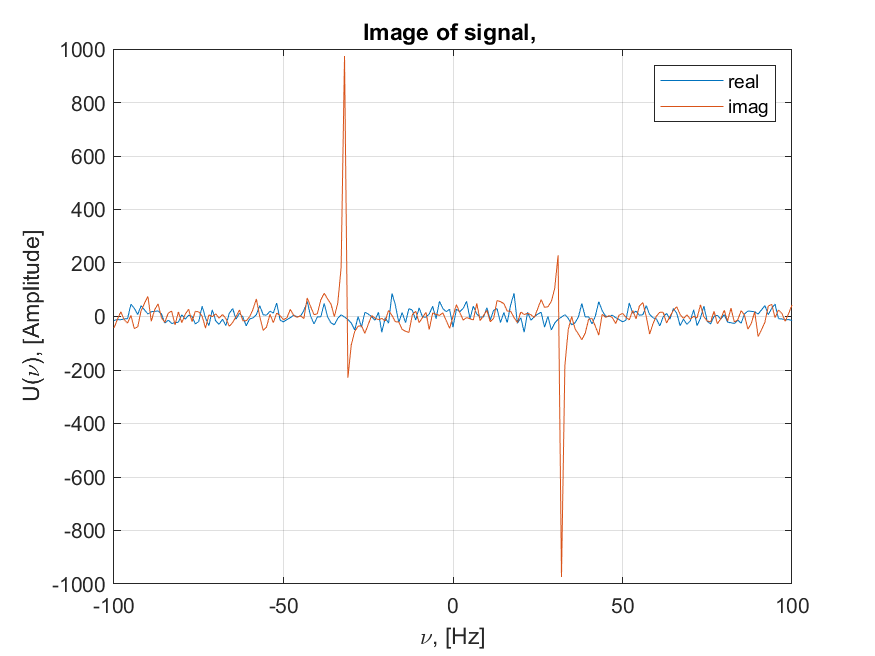
\includegraphics[width=0.7\textwidth]{image_of_numeric_diff_signal.png}
	\caption{Фурье-образ численной производной сигнала}
\end{figure}

\begin{figure}[ht]
    \centering
    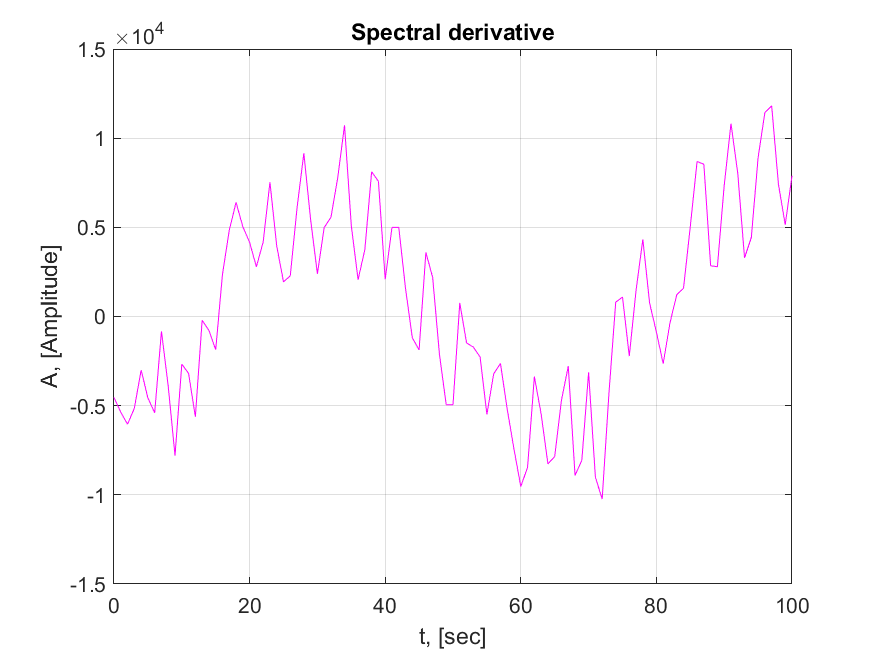
\includegraphics[width=0.7\textwidth]{spectral_diff.png}
	\caption{Спектральная производная}
\end{figure}

\newpage
\section{Графики для сравнения}

\begin{figure}[ht]
    \centering
    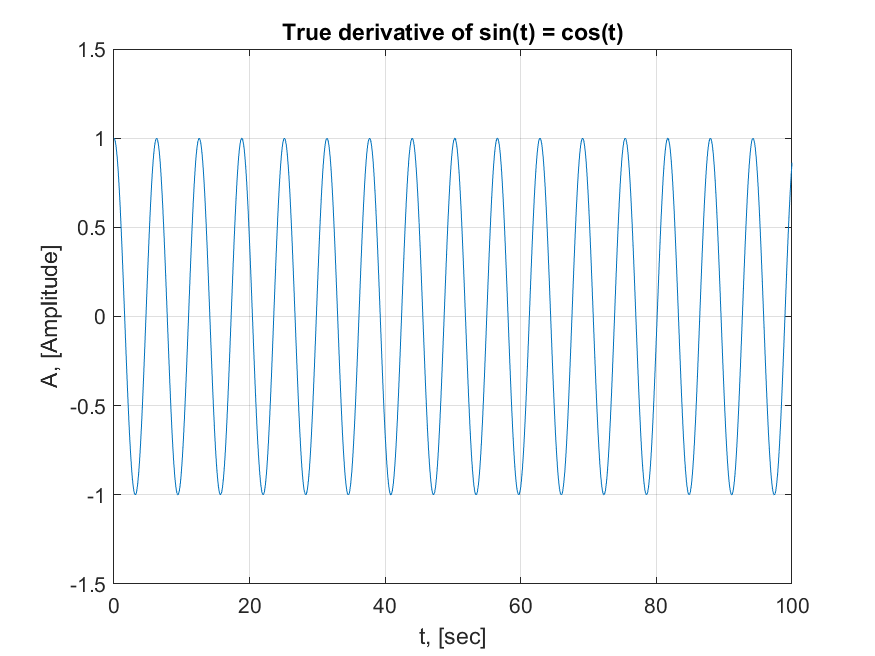
\includegraphics[width=0.7\textwidth]{true_diff.png}
	\caption{Истинная производная}
\end{figure}

\begin{figure}[ht]
    \centering
    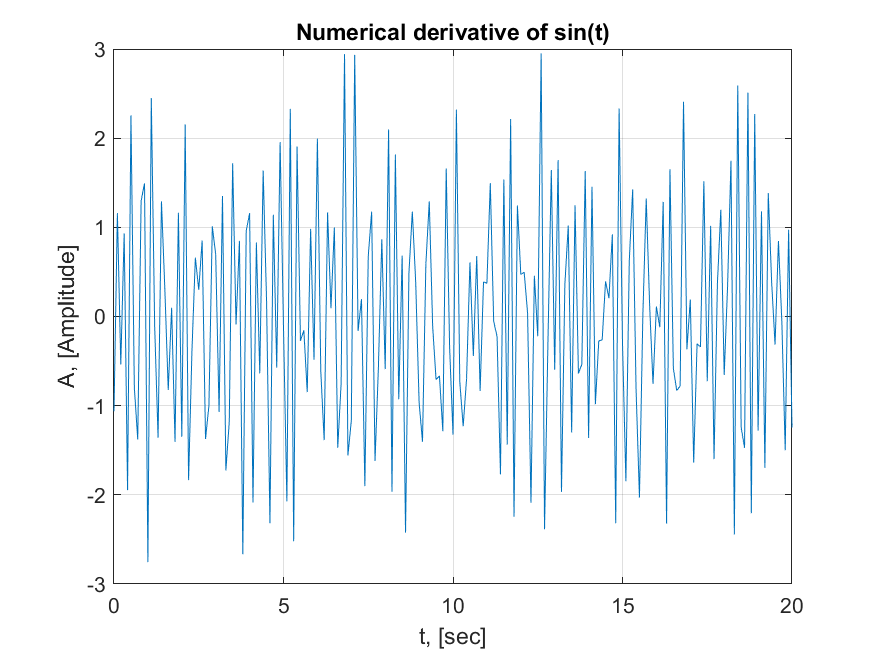
\includegraphics[width=0.5\textwidth]{numerical_diff.png}
	\caption{Численная производная}
\end{figure}

\begin{figure}[ht]
    \centering
    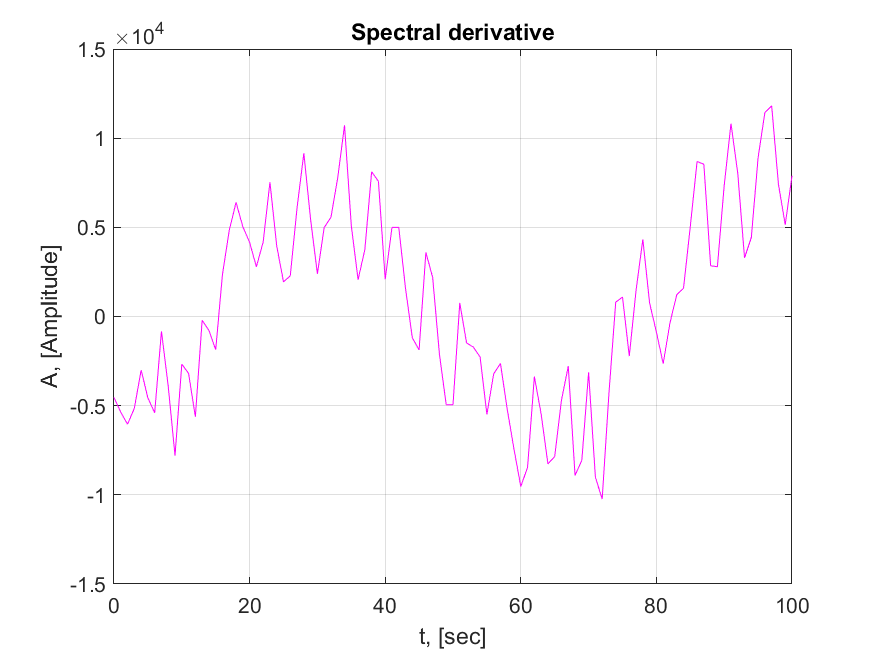
\includegraphics[width=0.7\textwidth]{spectral_diff.png}
	\caption{Спектральная производная}
\end{figure}

\newpage
\section{Делаем выводы}

Если не приближать и не рассматривать эти три графика вблизи, то кажется, что численная и спектральная - \textit{просто гармонический шум}... Если подобрать удачные отрезки рассмотрения, то прослеживается тот факт, что они очень сильно хотят напоминать график оригинальной производной, но не могут.
Думаю, что основное достижение сейчас - это то, что \textbf{мы смогли получить производную} без численного приближения только с помощью оператора Фурье и прямого, обратного преобразования.

\endinput